\documentclass[tikz, border=10pt]{standalone}
\usetikzlibrary{patterns}
\usepackage[outline]{contour}
\contourlength{0.09em}

\tikzset{
  nodeAll/.style={draw, rounded corners=3pt, text width=1.5em, align=center, thick},
  nodeA/.style={fill=black, text=white},
  nodeB/.style={fill=white, text=black, pattern=north east lines}
}

\begin{document}

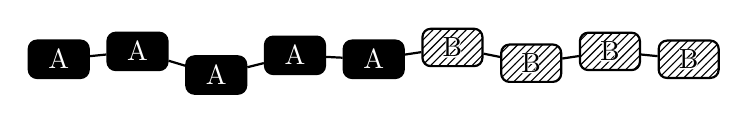
\begin{tikzpicture}
  \node[nodeAll, nodeA] (DBC-5) at (-5,0) {A};
  \node[nodeAll, nodeA] (DBC-4) at (-4,0.1) {A};
  \node[nodeAll, nodeA] (DBC-3) at (-3,-0.2) {A};
  \node[nodeAll, nodeA] (DBC-2) at (-2,0.05) {A};
  \node[nodeAll, nodeA] (DBC-1) at (-1,0) {A};
  \node[nodeAll, nodeB] (DBC0) at (0,0.15) {\contour{white}{B}};
  \node[nodeAll, nodeB] (DBC1) at (1,-0.05) {\contour{white}{B}};
  \node[nodeAll, nodeB] (DBC2) at (2,0.1) {\contour{white}{B}};
  \node[nodeAll, nodeB] (DBC3) at (3,0) {\contour{white}{B}};

  \path[thick]
    (DBC-5) edge (DBC-4)
    (DBC-4) edge (DBC-3)
    (DBC-3) edge (DBC-2)
    (DBC-2) edge (DBC-1)
    (DBC-1) edge (DBC0)
    (DBC0) edge (DBC1)
    (DBC1) edge (DBC2)
    (DBC2) edge (DBC3);
\end{tikzpicture}

\end{document}
